\subsection{Quản lý album ảnh}

Người dùng có thể quản lý, nhóm ảnh theo các album và xem danh sách các ảnh trong album đó như Hình \ref{fig:album}. Tại đây người dùng có thể xem danh sách các album đã tạo, tải album về máy hay xóa album.

\begin{figure}[H]
    \centering
    \begin{subfigure}{0.48\textwidth}
        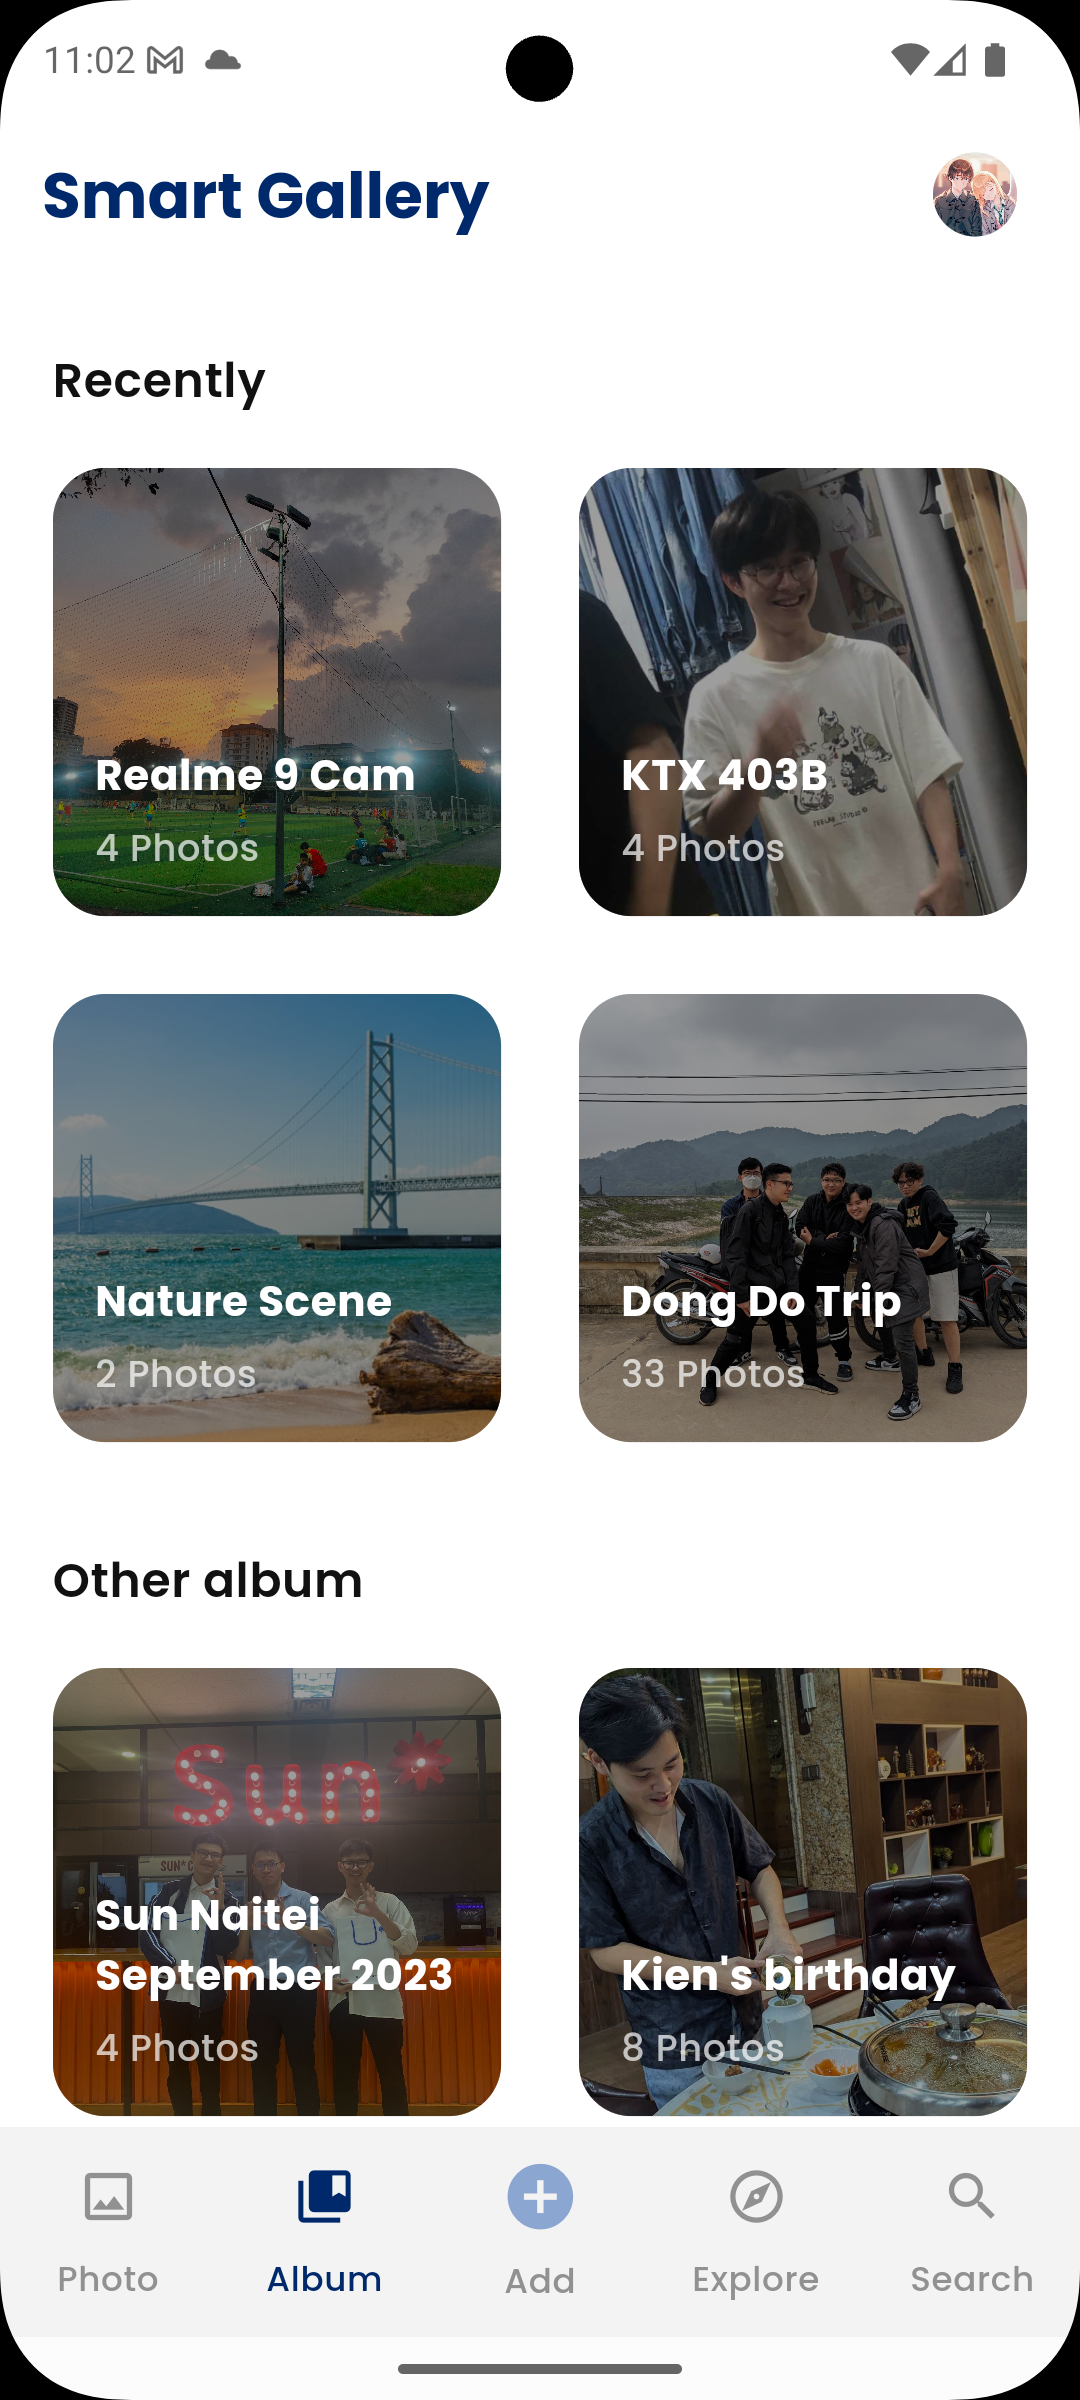
\includegraphics[width=1\linewidth]{figures/c4/4-2/album_1.png} 
        \caption{Danh sách album ảnh}
    \end{subfigure}
    \hfill
    \begin{subfigure}{0.48\textwidth}
        
\includegraphics[width=1\linewidth]{figures/c4/4-2/album_2.png} 
        \caption{Danh sách ảnh trong album}
    \end{subfigure}
    \caption{Giao diện album ảnh.}
    \label{fig:album}
\end{figure}

Hệ thống cung cấp giao diện tạo album với các ảnh người dùng đã tải lên hệ thống như Hình \ref{fig:create-album}

\begin{figure}[H]
    \centering  
    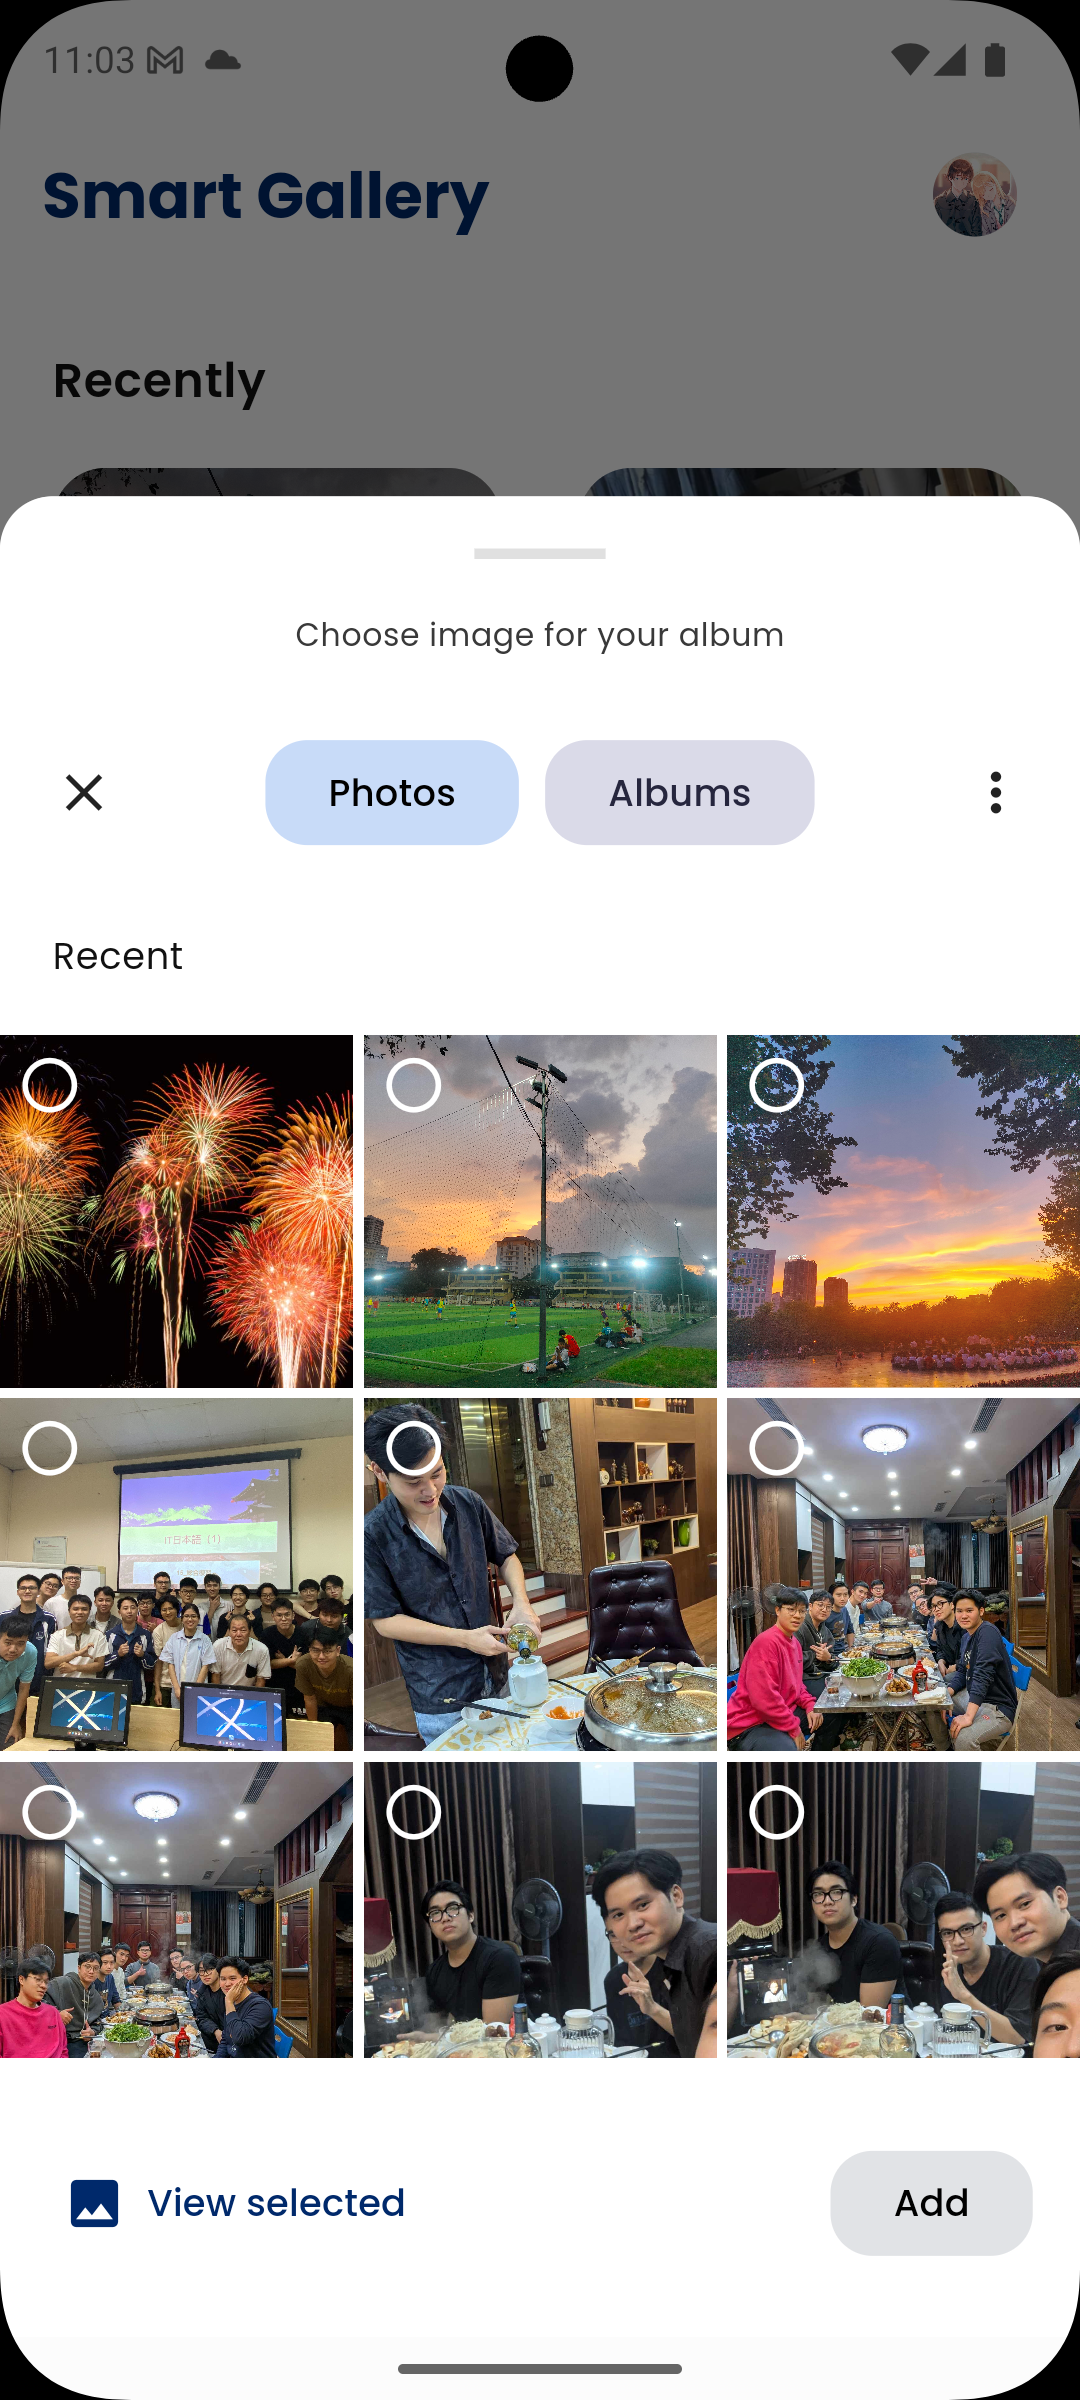
\includegraphics[width=0.5\textwidth]{figures/c4/4-2/create_album.png}
    \caption{Giao diện tạo album.}
    \label{fig:create-album}
\end{figure}